\chapter{STAGE 2: Booking}
\label{chap:book}
To start in this section, you must have been approved to book. If you are unsure of what that means, see STAGE 1: Apply To Book.
\begin{enumerate}
    \item Go to \href{https://bookings.venturercamp.org.uk}{\texttt{bookings.venturercamp.org.uk}}
    \item Click \verb|login|
    \begin{figure}[H]
        \centering
        \includegraphics[width=0.9\textwidth]{assets/login.png}
        \caption{Login Button}
    \end{figure}
    \item Login using the same service which you did last time (this is really important as otherwise, you'll have to apply to book again). The service which you used last time should be more \emph{vibrant} than the others.
    \begin{figure}[H]
        \centering
        \includegraphics[width=0.9\textwidth]{assets/login-using-vibrant.png}
        \caption{Login options with Login with Google highlighted}
    \end{figure}
    \item You will now be redirected back to the home page. Click \verb|Book|.
    \begin{figure}[H]
        \centering
        \includegraphics[width=0.9\textwidth]{assets/book.png}
        \caption{Book button}
    \end{figure}
    \item Now you will need to enter some details about the booking. Enter this information in the text boxes provided. You have the option to provide information about a second person should the team not be able to get in touch with you about the booking.
    \begin{figure}[H]
        \centering
        \includegraphics[width=0.9\textwidth]{assets/book-bookingSecDetails.png}
        \caption{Booking secretaries details}
    \end{figure}
    \item Scroll down to \verb|Participants|. Fill in that participants information. Participants will be listed on the right hand side of the screen underneath the \verb|Participants| header.
    \item To add additional participants, click the \verb|More People!| button. This will add another blank participant.
    \begin{figure}[H]
        \centering
        \includegraphics[width=0.2\textwidth]{assets/book-morePeople.png}
        \caption{More People! button}
    \end{figure}
    \item To remove a participant, click the cross button next to the attendance widget for that participant. You will then be prompted to confirm that you wish to remove that participant.
    \begin{figure}[H]
        \centering
        \includegraphics[width=0.9\textwidth]{assets/book-removeParticipant.png}
        \caption{Remove participant button}
    \end{figure}
    \item Scroll down to \verb|Money|. Here, you will be given a breakdown of the cost of your group to come to camp and payment instructions. We are only able to accept bank transfers, please select this option. See section \ref*{chap:payment} for more information on payment. When you are creating your booking for the first time, you will not have a payment reference. Once you submit your booking, a payment reference will be generated for you. 
    \item Continue scrolling down. If you have less than two over sixteen year olds in the booking, you will need to add the details of someone over 16 who can act as an emergency contact. This is done in the \verb|Emergency Contact| section. 
    \begin{figure}[H]
        \centering
        \includegraphics[width=0.9\textwidth]{assets/book-emergencyContact.png}
        \caption{Emergency Contact text boxes}
    \end{figure}
    \item Within \verb|Additional Information|, you are able to indicate if you are planning on using the shuttle coach services provided on the first and last day of camp to/ from Hereford Train Station, please delete the options you wish not to take as appropriate; and you can also indicate which groups you would like to camp with. We will take these requests on board however we cannot guarantee we will be able to meet all of them.
    \begin{figure}[H]
        \centering
        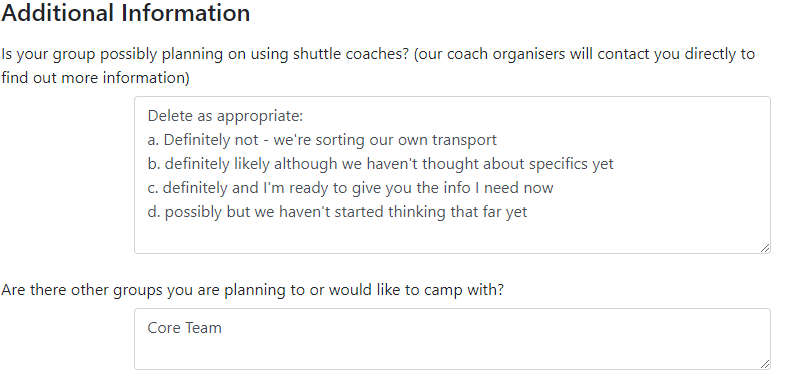
\includegraphics[width=0.9\textwidth]{assets/book-additionalInfo.png}
        \caption{Additional Information text boxes}
    \end{figure}
    \item When you have reviewed your booking and ticked the permission checkbox, the \verb|Submit Booking| button should un-grey-out. Click this to save the booking. Please ensure you see confirmation of the booking saving before you close the tab.\\
    The booking system won't let you submit your booking until enough information has been entered. A \verb|Still to do| box will indicate these things to you.
    \begin{figure}[H]
        \centering
        \includegraphics[width=0.9\textwidth]{assets/book-submit-stillToDo.png}
        \caption{Submit section showing outstanding tasks}
    \end{figure}
    \item Once you have clicked submit, you will be sent to a payment page where your invoice will be generated. This will also be emailed to you.
    \begin{figure}[H]
        \centering
        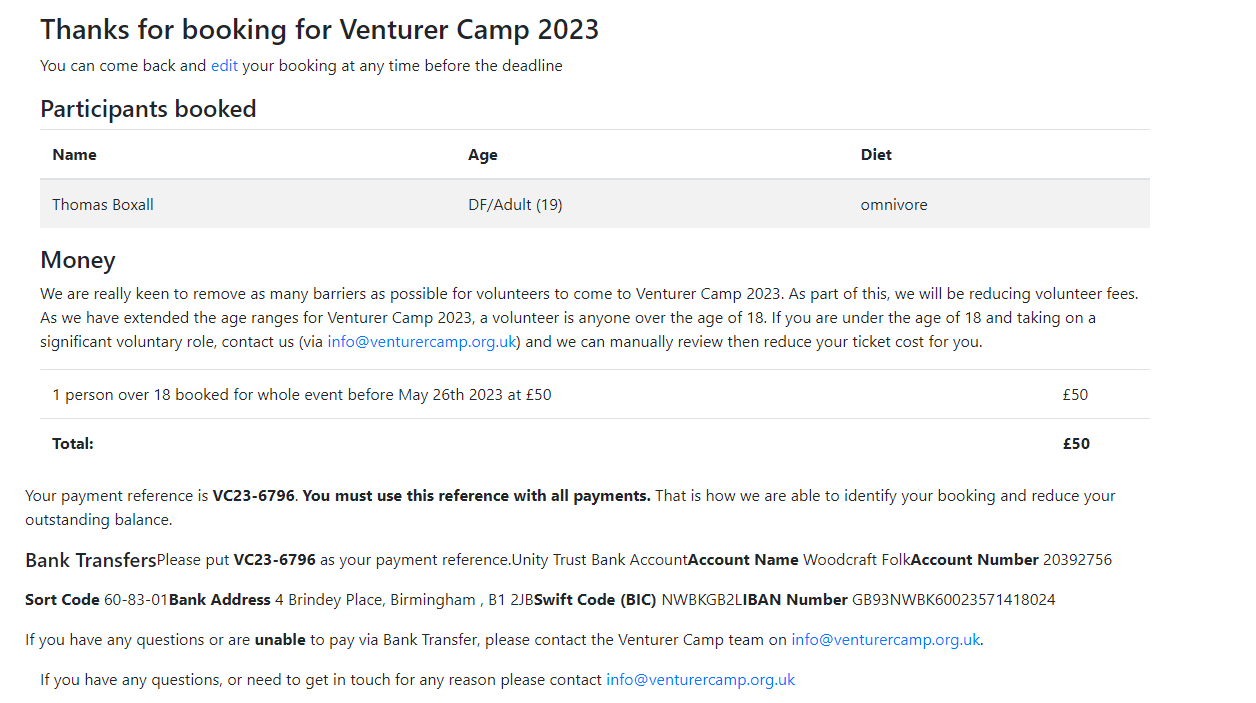
\includegraphics[width=0.9\textwidth]{assets/book-confirmation.png}
        \caption{Invoice page}
    \end{figure}
\end{enumerate}